\section{Case Studies}\label{sec:case-studies}
Let us begin by considering livelits from the client programmer's perspective by way of
two domain-specific case studies:
a course grade assignment case study in Sec.~\ref{sec:live-grading}
and an image transformation case study in Sec.~\ref{sec:image-transformation}.
% We also briefly mention several other examples in Sec.~\ref{sec:additional-examples}.\todo{do we?}{}
These case studies have been implemented
in Hazel, a browser-based live programming environment for a pure typed functional language in the
ML family. We assume basic familiarity with ML.

\subsection{Case Study: Grading with Livelits}\label{sec:live-grading}
\begin{figure}
    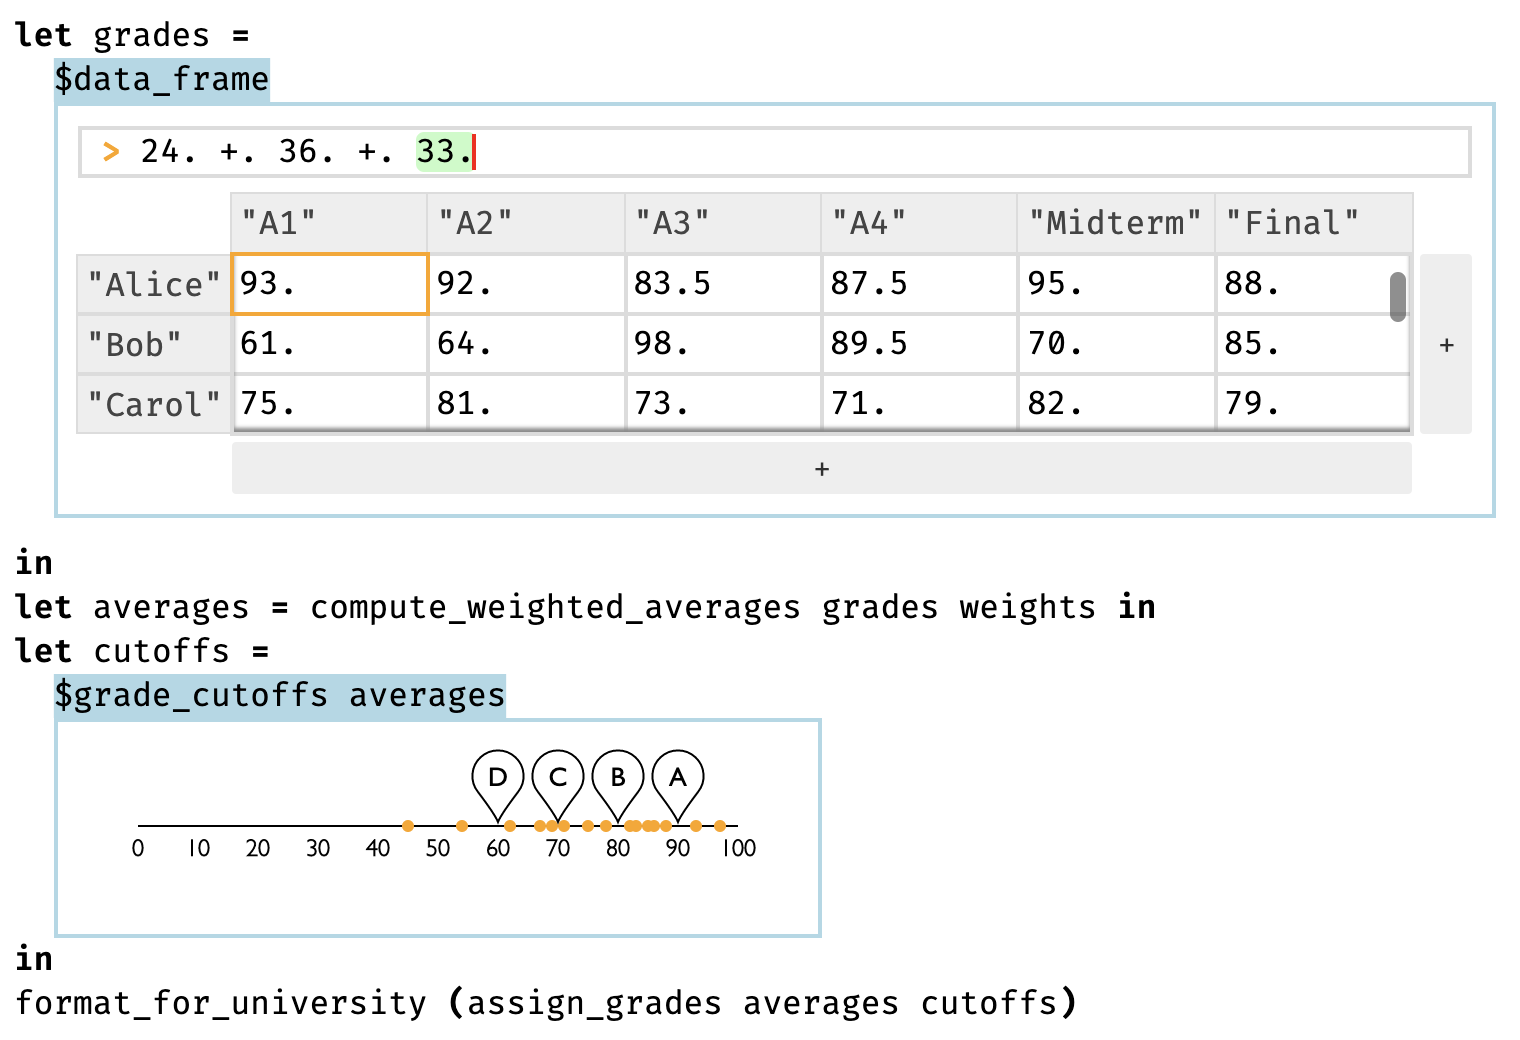
\includegraphics[width=30pc]{grade-cutoff-livelit.png}
\caption{Grading with Livelits}
\label{fig:grading}
\end{figure}

Consider this familiar scenario: an instructor needs
(1) to record numeric grades for various assignments and exams, and
(2) to visualize and perform various computations with these numeric grades
in order ultimately to assign final letter grades (\textbf{A} through \textbf{F}) to the students in the course.

Perhaps the most common end-user application in this domain is the spreadsheet.
A spreadsheet allows the instructor to record student grades using a natural tabular interface,
visualize this data in one of a finite number of plot styles, and perform basic computations on this data,
with results updated live, i.e. automatically after each cell has been edited.
However, these affordances are limited. It is difficult to package up common operations and workflows
into reusable libraries, interact with the data using domain-specific visualizations,
and perform operations that have not been anticipated by the designers of the spreadsheet system
(e.g. operations that prepare the data in an idiosyncratic format suitable for automated submission
to the university's grading system).
General-purpose programming languages equipped with suitable libraries for working with numeric data
are flexible enough to handle these scenarios, but users of these languages
sacrifice the ability to receive live feedback and directly manipulate data and visualizations thereof.

Livelits are able to address this tension.
Fig.~\ref{fig:grading} shows a Hazel program where the user has:
\begin{enumerate}
\item recorded numeric \li{grades} for each student using a livelit, \li{\$dataframe}, that implements a tabular user interface with support for live evaluation of the Hazel expression in each cell,
\item programmatically computed the overall \li{averages} for each student by applying a function, \li{compute_averages}, defined in a library  (not shown) shared between multiple courses,
\item determined reasonable \li{cutoffs} between letter grades by directly manipulating a livelit that offers a domain-specific drag-and-drop interface superimposed on a live visualization of the grade distribution
(for the sake of space, we plot dots rather than a full histogram),
\item programmatically assigned letter grades to each student based on the \li{cutoffs} determined in step (3) by calling another shared library function, \li{assign_grades},
\item formatted the final grade assignments in a manner suitable for submission to the university system by calling another shared library function, \li{format_for_university}.
\end{enumerate}

\subsubsection{Livelit Expansion}\label{sec:livelit-expansion}
Livelit expressions are given dynamic meaning by expansion to core expressions, i.e. expressions that do not contain livelits.
For example, the expansion of Fig.~\ref{fig:grading} is:

\begin{lstlisting}
let grades = Dataframe (
  ["A1", "A2", "A3", "A4", "Midterm", "Final"],
  [
    ("Alice", [24. +. 36. +. 33., 92., 83.5, 87.5, 95., 88.]),
    ("Bob", [61., 64., 98., 89.5, 70., 85.]),
    ("Carol", [75., 81., 73., 71., 82., 79.]),
    (* ... *)
  ]) in
let averages = compute_averages grades weights in
let cutoffs = (.A 90.0, .B 80.0, .C 70.0, .D 60.0) in
format_for_university (assign_grades averages cutoffs)
\end{lstlisting}

The programmer can inspect this expansion in Hazel.
Ideally, however, it would not be necessary to inspect the expansion
(or the livelit implementation, which specifies the expansion logic and is discussed in Sec.~\ref{sec:livelit-definitions})
to reason about types and binding.
After all, one does not need to look inside
function bodies to reason about types and binding.
Instead, in the words of \citet{DBLP:conf/ifip/Reynolds83},
``type structure is a syntactic discipline for maintaining levels of abstraction''.
The livelits mechanism supports reasoning abstractly about types and binding by
several means.

To support abstract reasoning about the type of the expansion,
livelit definitions declare an \emph{expansion type}.
The declarations of the two livelits in Fig.~\ref{fig:grading},
eliding their implementations, are:
\begin{lstlisting}[numbers=none]
livelit $dataframe at Dataframe { ... }
livelit $grade_cutoffs(avgs: List(Float))
  at (.A Float, .B Float, .C Float, .D Float) { ... }
\end{lstlisting}
The expansion type of \li{\$dataframe} is \li{Dataframe}
(a type classifying tabular floating point data together with string row and column keys, consistent with the expansion above)
and the expansion type of \li{\$grade_cutoffs} is a labeled product of grade cutoffs (Hazel notates labels \li{.label}).
Hazel summarizes the typing information from the livelit definition when the cursor is on the livelit's name,
just as it displays a function's type when its name is under the cursor (not shown).

\subsubsection{Typed Hygienic Splicing and Parameterization}\label{sec:splicing-and-parameterization}
Livelit expressions can include sub-expressions in one of two ways:
as parameters or as splices.

\paragraph{Parameters}\label{sec:parameterization} Parameters appear immediately after the name of the applied livelit.
For example, \li{averages} is provided as a parameter to \li{\$grade_cutoffs} in Fig.~\ref{fig:grading}.
The livelit declares a fixed number of parameters and specifies their types in its declaration.
For example, the declaration of \li{\$grade_cutoffs} shown above specifies one parameter of type \li{List(Float)}
(the grades data to be plotted, see below).

Livelit abbreviations can partially apply parameters. Consider the slider livelit
from Fig.~\ref{fig:color}:
\begin{lstlisting}[numbers=none]
livelit $slider (min: Float) (max: Float) at Float { ... }
\end{lstlisting}
We can partially apply the first parameter as follows to define a parameterized non-negative slider livelit with one remaining parameter:
\begin{lstlisting}[numbers=none]
livelit $nnslider = $slider 0.0 in ...
\end{lstlisting}
Only livelits with no remaining parameters can be used to fill a hole.
So writing \li{\$nnslider} in expression position will not display the slider GUI. Instead, it will display as a ``missing livelit parameter'' error.%
\footnote{\label{footnote:typing}In Hazel, erroneous expressions are automatically placed inside holes so that they do not prevent other parts of the program from executing
\cite{HazelnutLive}.}

\paragraph{Splices}\label{sec:splices}
Spliced expressions (or \emph{splices}) appear directly inside the livelit GUI.
Splices can be filled with Hazel expressions of any form, including other livelit expressions,
and all of Hazel's editing affordances are available when editing these expressions.
For example, each cell in the \li{\$dataframe} GUI in Fig.~\ref{fig:grading}
has a corresponding splice, which appears in the formula bar at the top of the livelit
when the user has selected that cell.
The cell itself displays the live value of the spliced expression,
following the example of spreadsheet interfaces
(we return to live evaluation in Sec.~\ref{sec:live-evaluation} below).

The livelit provides an expected type for each splice.
For example, the splices for the row and column keys in Fig.~\ref{fig:grading} are expected to be expressions
of type \li{String}, and the remaining cells are expected to be expressions of type \li{Float}.
Hazel surfaces this typing information for the programmer when the cursor is in a splice,
so it is not necessary to inspect the expansion or the livelit implementation.
If an expression of invalid type is entered, it will display in an error hole as usual,
and in Hazel this will not prevent evaluation of other expressions (see Footnote \ref{footnote:typing}).

Unlike parameters, the number of splices is not fixed in the livelit declaration. Splices can be created,
deleted, and filled through user interaction with the livelit. For example, clicking the \li{+} buttons
in Fig.~\ref{fig:grading} will create new rows or columns, which will in turn generate new splices.

\paragraph{Hygiene}\label{sec:hygiene}
Parameters and splices can both appear in the expansion. For example,
the expansion of the \li{\$dataframe} livelit in Fig.~\ref{fig:grading} includes the
entered cell contents and the row and column keys.

The client cannot know, without looking at the expansion or the livelit implementation,
where in the expansion each parameter or splice will appear. This becomes relevant when
the expansion places the parameter or splice under a binder, e.g. in the body of a function or let binding.
Na\"ively, this could cause inadvertent capture of the bound variable by a free variable
in the parameter or splice. For example, consider a livelit that generates an expansion
of the following form:
\begin{lstlisting}[numbers=none]
let len = strlen <splice1> in
(<splice2>, <splice2> + 1)
\end{lstlisting}
Here, \li{<splice2>} appears under the binding of \li{len}. If the client's choice for
\li{<splice2>} itself refers to a client-side binding of the same identifier, \li{len},
it would na\"ively be captured. This sort of bug would difficult to debug,
both for the livelit provider and the client.

To avoid this situation, the livelit expansion mechanism
maintains parameter and splice hygiene: parameters and splices are included in the expansion
in a capture-avoiding manner.
Consequently, clients can reason abstractly about binding in splices: variables in splices
always refer to bindings visible to the client, rather than bindings that are hidden inside expansions.
% This is implemented by alpha-renaming bindings internal to the expansion as necessary.
% (We discuss potentially relaxed variations of this hygiene discipline in Sec.~\ref{sec:discussion}.)

\subsubsection{Live Evaluation}\label{sec:live-evaluation}
Livelits can request the result of evaluating a splice or a parameter.
For example, the \li{\$dataframe} livelit uses this facility to display
the evaluation result for each cell when the cursor is not on it, like a spreadsheet.
The \li{\$grade_cutoffs} livelit uses this facility to plot the grades list, provided
as a parameter, on the number line.

\paragraph{Closure Collection} Evaluation in Hazel is, as usual, defined only for closed expressions,
but parameters and splices can both refer to variables in the surrounding
context. In order to provide evaluation results for parameters or splices containing free variables,
Hazel performs \textbf{closure collection} in two phases.

In the first phase, Hazel evaluates the program after placing holes in place of each livelit,
following the evaluation semantics for incomplete programs developed by \citet{HazelnutLive}.
The result is an expression with holes in it, each of which is equipped with a closure.
For example, there is a single closure associated with the application of \li{\$dataframe} in Fig.~\ref{fig:grading}.
This closure contains the value of the \li{weights} variable from Line 1 and any other variables in the context
around that livelit, e.g.
from imported libraries, not shown. Consequently, when the livelit requests the evaluation result for
splices that use these variables, such as the cell shown selected in Fig.~\ref{fig:grading},
an evaluation result is available. (We consider the situation where more than one closure is available
in the Sec.~\ref{sec:image-transformation}.)

Similarly, the closure for the \li{\$grade_cutoffs} livelit in Fig.~\ref{fig:grading} includes a result for
the \li{grades} variable. However, this variable's result, along with the
results for other variables that depend on \li{grades}, such as \li{averages}, ultimately depend on the
expansion of the \li{\$dataframe} livelit. If we stop after the first phase of closure collection,
where these expansions have not yet been included,
then no useful result will be available here.
For this reason, there is a second phase of closure collection where any livelit holes that appear
in the collected livelit closures are \emph{resumed}, i.e. the expansion is generated
(in this case, for the \li{\$dataframe} livelit) and is used to fill
the hole before evaluation resumes, following the semantics for resumption developed by \citet{HazelnutLive}.
Livelit expansions do not themselves contain livelits, so no subsequent resumption phases are necessary.

The final evaluation result for the program as a whole can also proceed by resumption, because
closure collection performs all of the computations that do not ultimately depend on the livelit expansion.
Consequently, Hazel does not need to evaluate the program multiple times in order to support edit-time
(i.e. live) evaluation in this way.

\paragraph{Indeterminate Results}
We used the phrase \emph{evaluation result} rather than \emph{value} above purposefully:
splices and parameters can be incomplete, i.e. they can contain holes, so
evaluation does not always result in a value \cite{HazelnutLive}.
In particular, when a hole appears in elimination position, e.g. in function position of a function application,
 the result is instead an indeterminate expression.
When a livelit requests an evaluation result, it must be able to handle indeterminate results.
For example, if the parameter to \li{\$grade_cutoffs} were a hole or some other indeterminate expression,
then it would have degraded functionality
(in this case, it would display the list elements that are values on the timeline, skipping indeterminate elements).
We will return to how livelit implementations handle this situation in Sec.~\ref{sec:livelit-definitions}.

\subsection{Case Study: Image Transformations}\label{sec:image-transformation}

\begin{figure*}
  \begin{center}
    \begin{subfigure}[t]{0.5\textwidth}
      \centering
      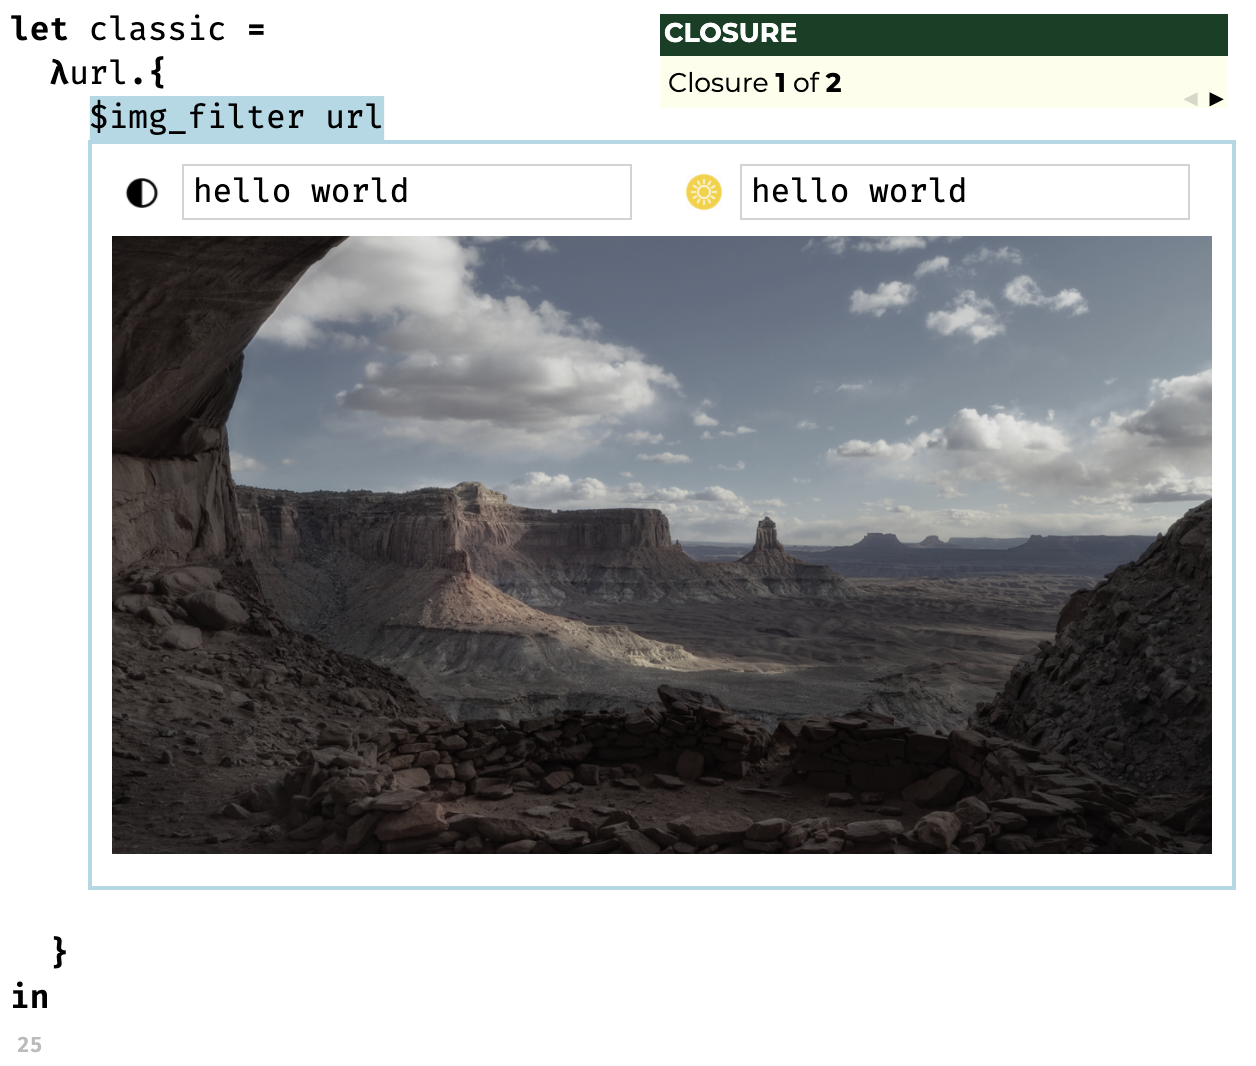
\includegraphics[width=15pc]{img-filter-1.png}
      \caption{}
    \end{subfigure}\begin{subfigure}[t]{0.5\textwidth}
      \centering
      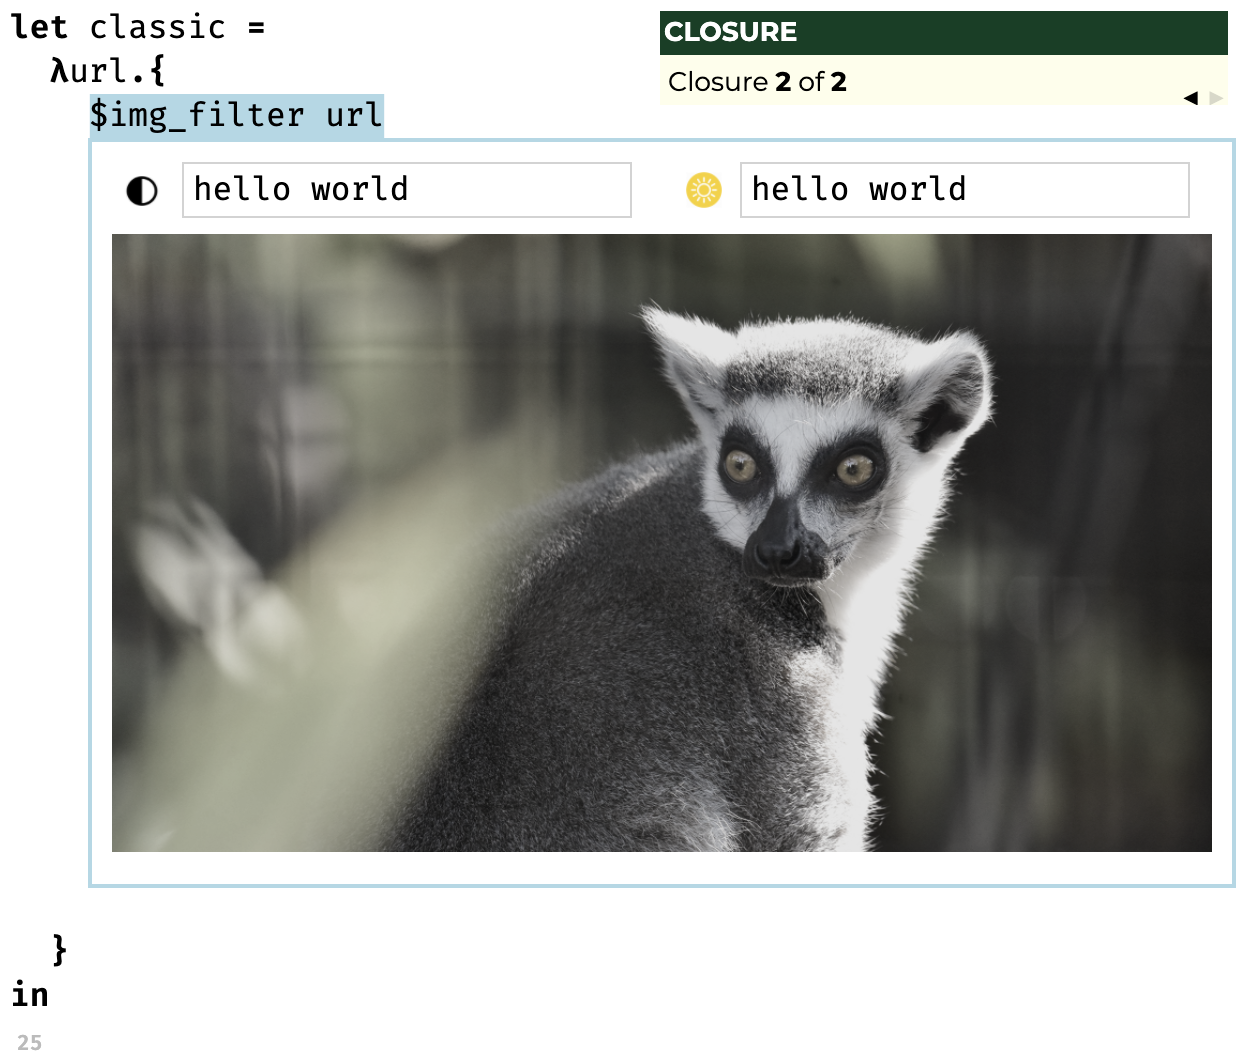
\includegraphics[width=15pc]{img-filter-2.png}
      \caption{}
    \end{subfigure}
  \end{center}
  \caption{hello world}
  \label{fig:color}
\end{figure*}

Show example of an image transformation pipeline going through livelits

This might also benefit from Parameterization

Show multiple calls with different example images + closure selector UIs

Go into more detail about how evaluation works + fill-and-resume mechanics (and efficiency nod)

Talk about probes?

We assume that the user has selected at most one closure for each livelit in the unexpanded expression.
The corresponding environment is applied as a substitution before attempting to evaluate the requested expression.
To maintain the context independence principle, this request must take the form of a closed function
of the splices.
As discussed in Sec.~\ref{sec:live-evaluation}, evaluation can fail if the free variables in the splices
overlap with the free variables in selected closure.

% \subsection{Additional Examples}\label{sec:additional-examples}
% It would be nice to have a gallery-style figure and a brief overview of some other case studies
% and how they exercise the novel features of the livelits mechanism. Maybe some statistics on how
% many lines of code it took.

% Ideas:
% \begin{itemize}
%   \item derivation trees like Joomy's system (\url{https://joom.github.io/proof-tree-builder/src/})
% \end{itemize}